\documentclass[border=10pt]{standalone}
\usepackage{pgfplots}
\usepgfplotslibrary{colormaps}
\pgfplotsset{trig format plots=rad}
\begin{document}
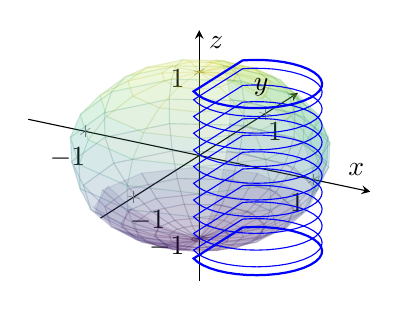
\begin{tikzpicture}
\begin{axis}[
    view={30}{30},
    xmin=-1.5, xmax=1.5,
    ymin=-1.5, ymax=1.5,
    zmin=-1.5, zmax=1.5,
    axis lines=center,
    xlabel=$x$, ylabel=$y$, zlabel=$z$,
    grid=major,
]
% Sphere: x^2 + y^2 + z^2 = 1
\addplot3[surf, opacity=0.1, domain=0:3.14159, y domain=0:6.28318, samples=15, colormap/viridis] 
    ({sin(deg(x))*cos(deg(y))}, {sin(deg(x))*sin(deg(y))}, {cos(deg(x))});

% Cylinder: r = cos(theta)
% Using a simpler approach: a series of circles
\foreach \z in {-0.9,-0.7,...,0.9} {
    \addplot3[domain=-1.57:1.57, samples=30, thin, blue] 
        ({cos(deg(x))^2}, {cos(deg(x))*sin(deg(x))}, \z);
}
\addplot3[domain=-1.57:1.57, samples=30, thick, blue] 
    ({cos(deg(x))^2}, {cos(deg(x))*sin(deg(x))}, 1);
\addplot3[domain=-1.57:1.57, samples=30, thick, blue] 
    ({cos(deg(x))^2}, {cos(deg(x))*sin(deg(x))}, -1);

\end{axis}
\end{tikzpicture}
\end{document}
